%%%%%%%%%%%%%%%%%%%%%%%%%%%%%%%%%%%%%%%%%%%%%%%%%%%%%%%%%%%%%%%%%%%%%%
% Overleaf (WriteLaTeX) Example: Molecular Chemistry Presentation
%
% Source: http://www.overleaf.com
%
% In these slides we show how Overleaf can be used with standard 
% chemistry packages to easily create professional presentations.
% 
% Feel free to distribute this example, but please keep the referral
% to overleaf.com
% 
%%%%%%%%%%%%%%%%%%%%%%%%%%%%%%%%%%%%%%%%%%%%%%%%%%%%%%%%%%%%%%%%%%%%%%

\documentclass{beamer}

\mode<presentation>
{
  \usetheme{Madrid}       % or try default, Darmstadt, Warsaw, ...
  \usecolortheme{default} % or try albatross, beaver, crane, ...
  \usefonttheme{default}    % or try default, structurebold, ...
  \setbeamertemplate{navigation symbols}{}
  \setbeamertemplate{caption}[numbered]
} 

\usepackage[english]{babel}
\usepackage[utf8x]{inputenc}
\usepackage{graphicx}
\usepackage{hyperref}
  \hypersetup{colorlinks=true}
  \hypersetup{urlcolor=blue}
  \hypersetup{linkcolor = .}
\usepackage{xcolor}
\usepackage{siunitx}
  \sisetup{separate-uncertainty = true}
\usepackage{physics}
\usepackage[font=small,labelfont=bf]{caption}
\usepackage{subcaption}
\usepackage[en-GB]{datetime2}
\usepackage{overpic}
\usepackage{feynmp}
\DeclareGraphicsRule{*}{mps}{*}{}
\usepackage{scalerel}
\newcommand{\mylbrace}[2]{\vspace{#2pt}\hspace{6pt}\scaleleftright[\dimexpr5pt+#1\dimexpr0.06pt]{\lbrace}{\rule[\dimexpr2pt-#1\dimexpr0.5pt]{-4pt}{#1pt}}{.}}
\newcommand{\myrbrace}[2]{\vspace{#2pt}\scaleleftright[\dimexpr5pt+#1\dimexpr0.06pt]{.}{\rule[\dimexpr2pt-#1\dimexpr0.5pt]{-4pt}{#1pt}}{\rbrace}\hspace{6pt}}

% Here's where the presentation starts, with the info for the title slide
\title[$K^+K^-\pi^+\pi^-$]{Update on \texorpdfstring{$B^\pm\to Dh^\pm$}{B to Dh}, \texorpdfstring{$D\to K^+K^-\pi^+\pi^-$}{K+K-pi+pi-} analysis at LHCb and BESIII}

\author{Martin Tat}
\institute{Oxford LHCb}
\date{10th January 2022}

\titlegraphic{
\includegraphics[height = 2cm]{lhcb.jpg}\hspace{1cm}~%
              
\includegraphics[height = 2cm]{OxfordLogo.pdf}\hspace{1cm}~%
              
\includegraphics[height = 2cm]{bes3.jpg}}

\begin{document}

\begin{frame}
  \titlepage
\end{frame}

% These three lines create an automatically generated table of contents.
\begin{frame}{Outline}
  \tableofcontents
\end{frame}

\section{LHCb}
\subsection{Summary of current LHCb analysis progression}

\begin{frame}{LHCb analysis summary}
  \begin{itemize}
    \setlength\itemsep{0.5em}
    \item{Previous report on $B^\pm\to Dh^\pm$, $D\to K^+K^-\pi^+\pi^-$:}
    \begin{enumerate}
      \setlength\itemsep{0.5em}
      \item{Global mass fit $\implies$ Obtain mass shape}
      \item{Binned CP fit $\implies$ Obtain CP observables}
      \item{Backgrounds: Charmless, $D\to K\pi\pi\pi\pi^0$, $D\to K\pi\pi\pi$, $D\to K(X)l\nu$}
      \item{Systematic uncertainties: Mostly $c_i$, $s_i$}
    \end{enumerate}
  \end{itemize}
  \begin{figure}
    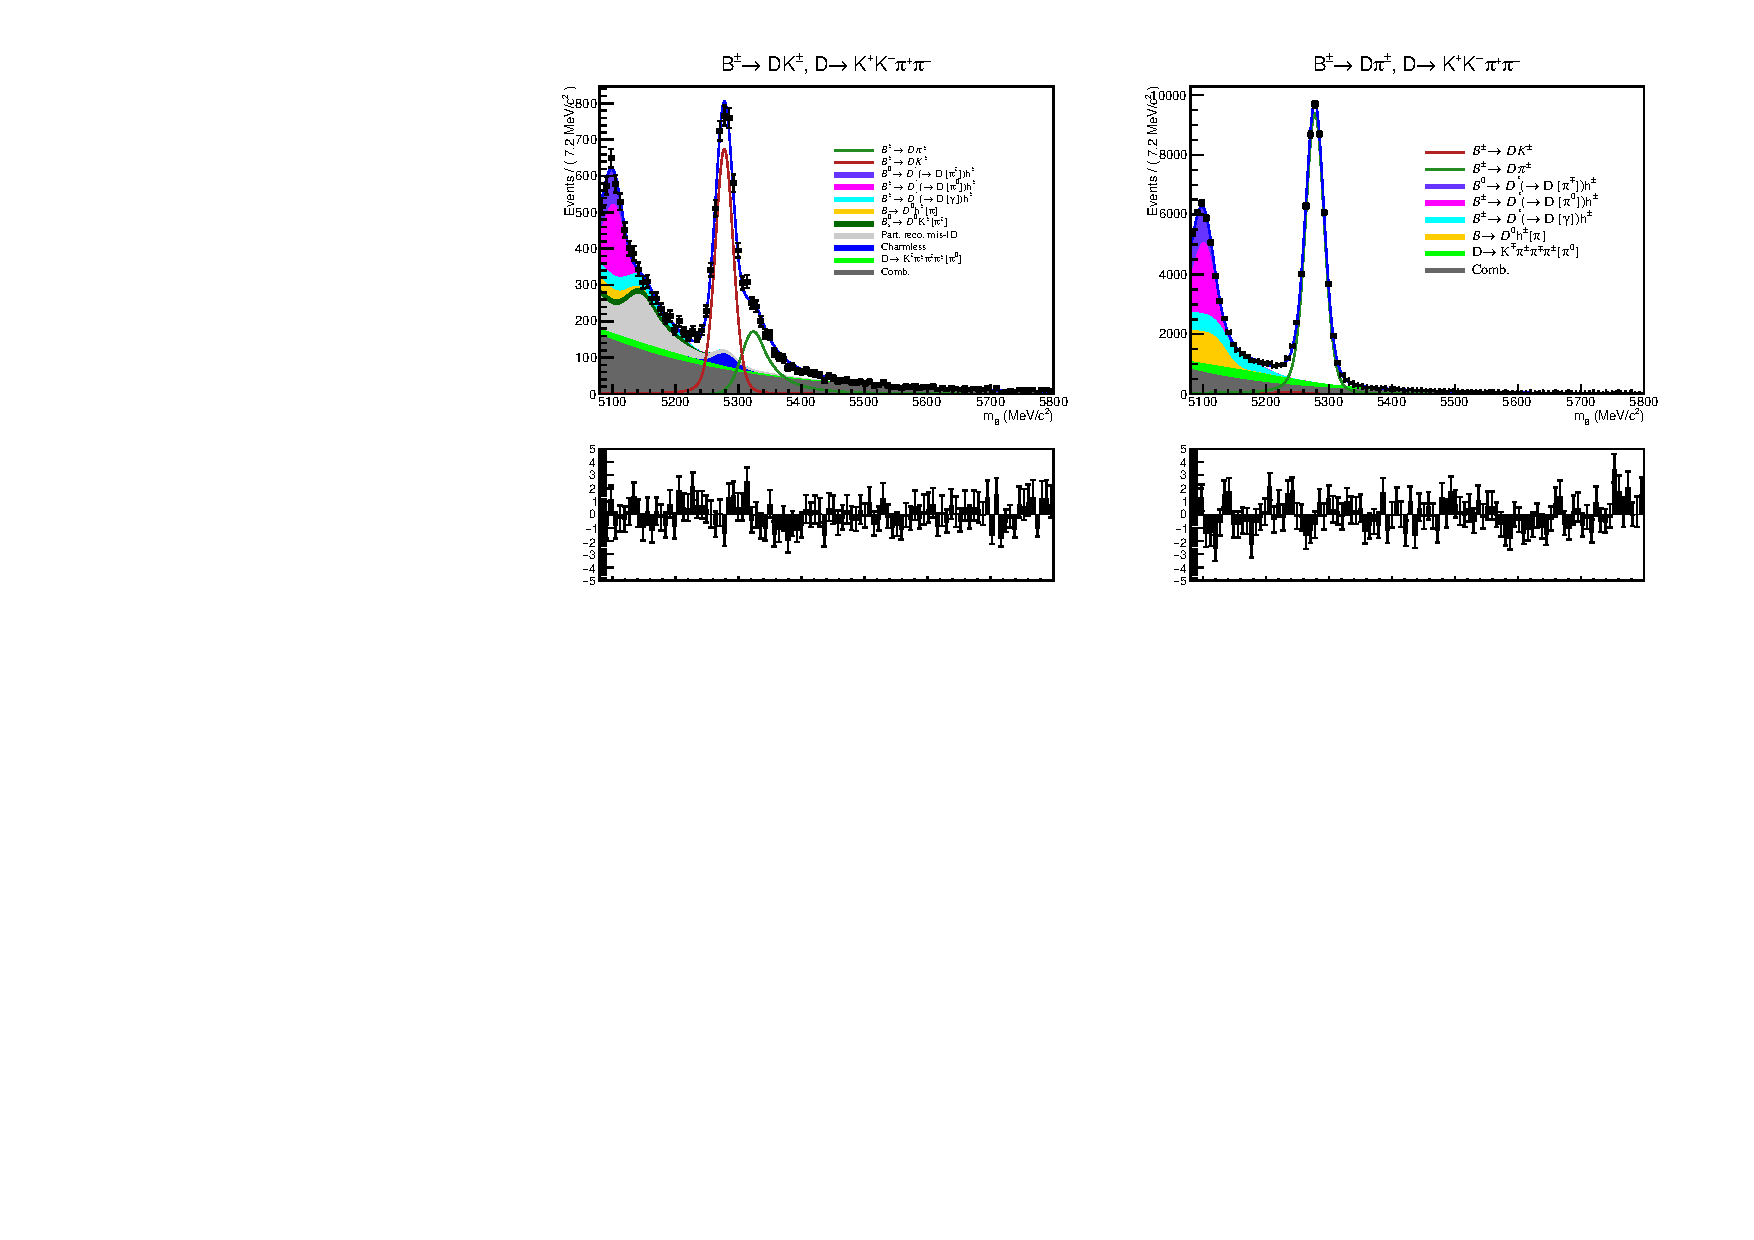
\includegraphics[width = 0.85\textwidth]{Plots/d2kkpipi_fiveL_allDP.pdf}
  \end{figure}
\end{frame}

\begin{frame}{LHCb analysis summary}
  \begin{itemize}
    \setlength\itemsep{0.5em}
    \item{Current analysis progress:}
    \begin{enumerate}
      \setlength\itemsep{0.5em}
      \item{Finished ANA note draft, currently in 1st circulation in B2OC WG}
      \item{Received comments from 2/3 reviewers, replies ready this week}
      \begin{itemize}
        \item{Will request $B\to(K\pi\pi\pi\pi^0)_Dh^\pm$ MC}
        \item{Fit with $c_i$, $s_i$ floated?}
      \end{itemize}
      \item{Need to finish off systematics for:}
      \begin{itemize}
        \item{Charmless and $K\pi\pi\pi\pi^0$ backgrounds}
        \item{$c_i$, $s_i$ model-dependent uncertainties}
      \end{itemize}
    \end{enumerate}
  \end{itemize}
  \begin{figure}
    \centering
    \vspace{-0.2cm}
    \begin{subfigure}{0.30\textwidth}
      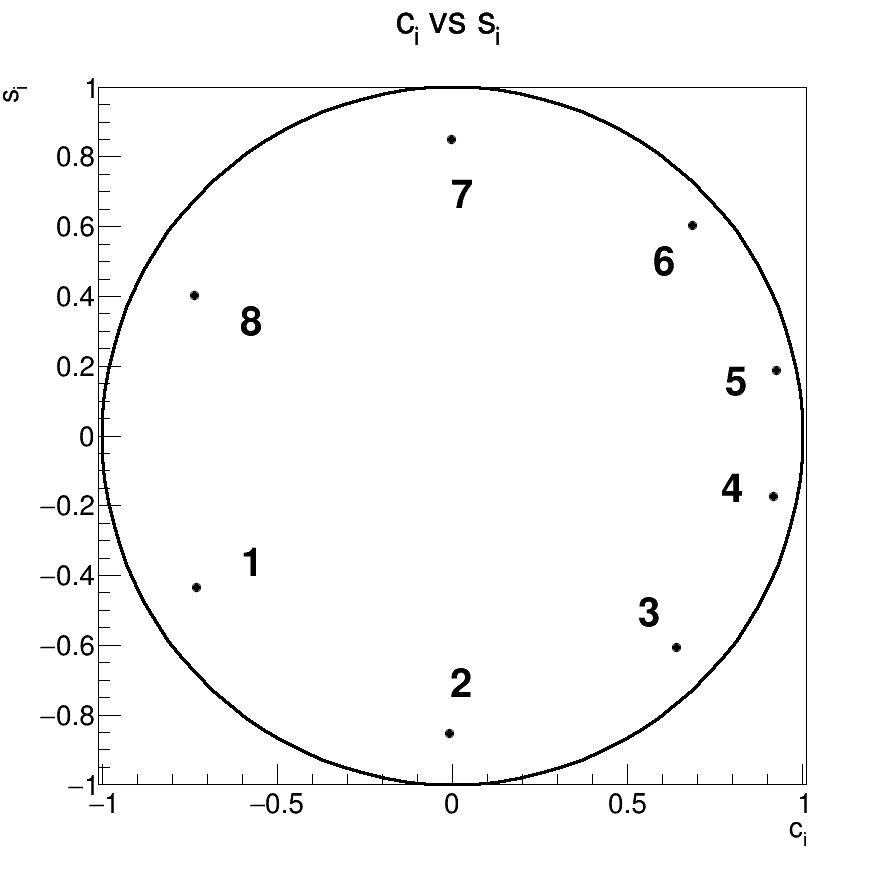
\includegraphics[width = 1.0\textwidth]{Plots/StrongPhaseParametersPlot_cisi_8Bins.png}
      \caption{LHCb model}
    \end{subfigure}%
    \begin{subfigure}{0.30\textwidth}
      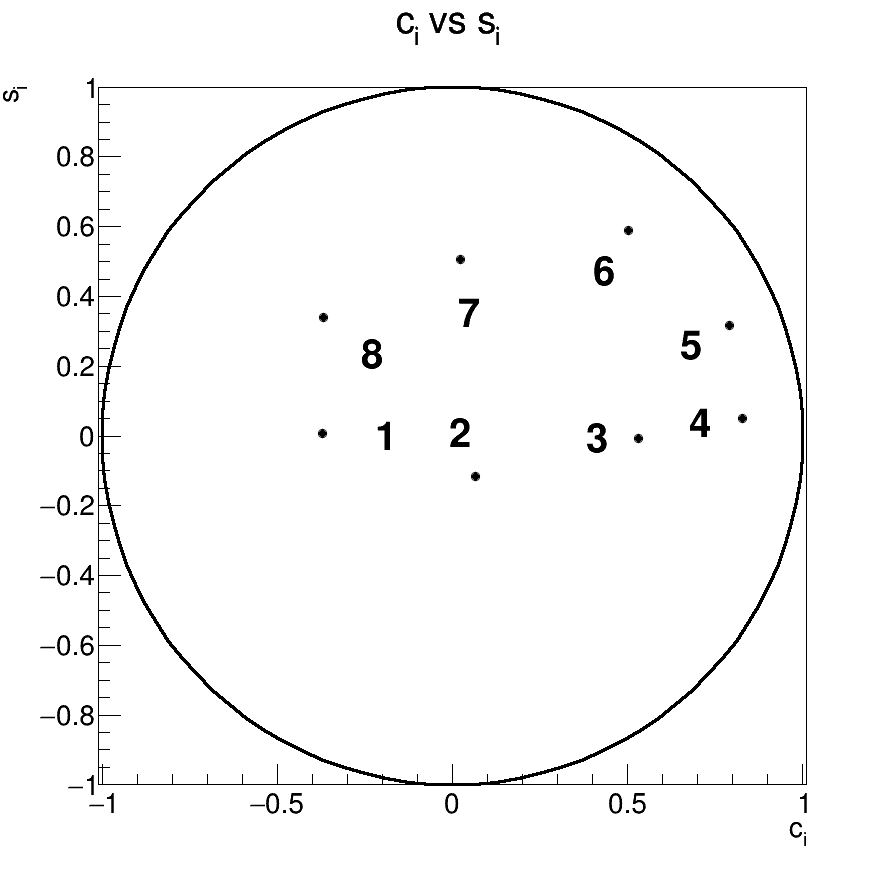
\includegraphics[width = 1.0\textwidth]{Plots/StrongPhaseParametersPlot_Mint2_cisi_8Bins.png}
      \caption{CLEO model}
    \end{subfigure}
  \end{figure}
\end{frame}

\section{BESIII}
\subsection{Strong-phase determination in quantum correlated \texorpdfstring{$D^0\bar{D^0}$}{D0D0} decays}

\begin{frame}{Strong-phase determination in quantum correlated $D^0\bar{D^0}$ decays}
  \begin{itemize}
    \item{BESIII: $e^+e^-$ collider at $\psi(3770)\to D^0\bar{D^0}$ threshold}
    \begin{itemize}
      \item{2010-2011: $\SI{2.93}{\per\femto\barn}$}
      \item{Since 23rd December: $\SI{0.46}{\per\femto\barn}$}
      \item{Expect $\SI{20}{\per\femto\barn}$ by end of 2023}
    \end{itemize}
  \end{itemize}
  \begin{figure}
    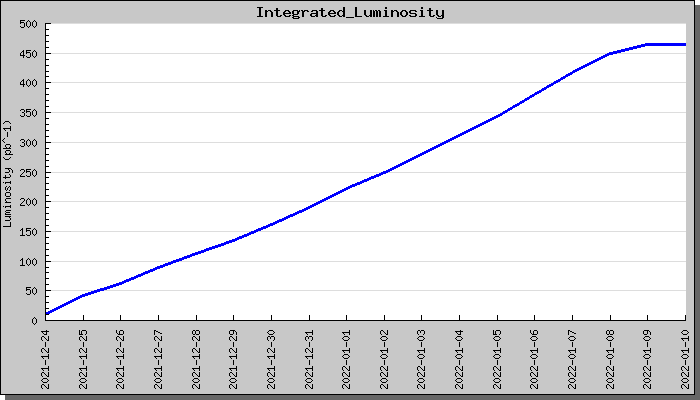
\includegraphics[width = 0.70\textwidth]{Plots/BES3_Integrated_Luminosity.png}
  \end{figure}
\end{frame}

\begin{frame}{Strong-phase determination in quantum correlated $D^0\bar{D^0}$ decays}
  \begin{itemize}
    \item{$D^0\bar{D^0}$ pair is quantum correlated}
  \end{itemize}
  \begin{figure}[H]
    \centering
    \vspace{-1.5cm}
    \begin{fmffile}{fgraph/fgraph_ee1}
      \setlength{\unitlength}{1cm}
      \begin{fmfgraph*}(8,5)
        \fmfleft{i}
        \fmfright{o}
        \fmflabel{$D^0$}{i}
        \fmflabel{$\bar{D^0}$}{o}
        \fmf{fermion}{w,i}
        \fmf{fermion}{w,o}
        \fmfblob{1cm}{w}
        \fmfv{label=$\psi(3770)$,label.dist=15,label.angle=90}{w}
      \end{fmfgraph*}
    \end{fmffile}
    \vspace{-1.5cm}
  \end{figure}
  \begin{itemize}
    \item{Equivalently, we can consider $D_+D_-$}
    \begin{itemize}
      \item{$D_\pm = \frac{1}{\sqrt{2}}(D^0\pm\bar{D^0})$ are CP eigenstates}
    \end{itemize}
  \end{itemize}
  \begin{figure}[H]
    \centering
    \vspace{-1.5cm}
    \begin{fmffile}{fgraph/fgraph_ee2}
      \setlength{\unitlength}{1cm}
      \begin{fmfgraph*}(8,5)
        \fmfleft{i}
        \fmfright{o}
        \fmflabel{$D_+$}{i}
        \fmflabel{$D_-$}{o}
        \fmf{fermion}{w,i}
        \fmf{fermion}{w,o}
        \fmfblob{1cm}{w}
        \fmfv{label=$\psi(3770)$,label.dist=15,label.angle=90}{w}
      \end{fmfgraph*}
    \end{fmffile}
    \vspace{-1.5cm}
  \end{figure}
\end{frame}

\subsection{First look at binned fits: Measurement of fractional bin yields \texorpdfstring{$K_i$}{Ki}}

\subsection{Measurement of CP-even fraction \texorpdfstring{$F_+$}{F+}}

\section{Summary and conclusion}
\begin{frame}{Summary and conclusion}
  \begin{center}
    {\huge Summary and conclusion}
  \end{center}
\end{frame}

\begin{frame}{Summary of CP observables}
  \begin{itemize}
    \item{}
  \end{itemize}
\end{frame}

\end{document}
